\chapter{Real-time scheduling algorithms}
I task possono essere schedulati i task in base alla \textit{deadline}, che può essere quella \textbf{relativa} o \textbf{assoluta}.

\section{Earlies Due Date}
Esegue come primo task quello con la \textit{deadline} relativa più immeinente.
\begin{itemize}
    \item tutti i taks arrivano simulataneamente.
    \item priorità fissati\item i task sono \textit{preemptabili}.
    \item permette di minimizzare la massima \textbf{\textit{lateness}} $L_i$ $\rightarrow$ nessun task manca la sua \textit{deadline}.
\end{itemize}
\begin{center}
    \begin{math}
        \begin{cases}
            L_i = f_i - d_i \qquad f_i \text{ è il finish time e } d_i \text{ è la deadline} \\
            L_{max} = \max_i(L_i)
        \end{cases}
    \end{math}
\end{center}

\newpage

\textcolor{green}{\textbf{Dimostrazione dell'ottimalità di EDD}}: consideriamo uno scheduler $\sigma \neq$ EDD e un'altro scheduler $\sigma'$ che è uguale a EDD fino all'istante $f_a$.
\begin{figure}[h]
    \centering
    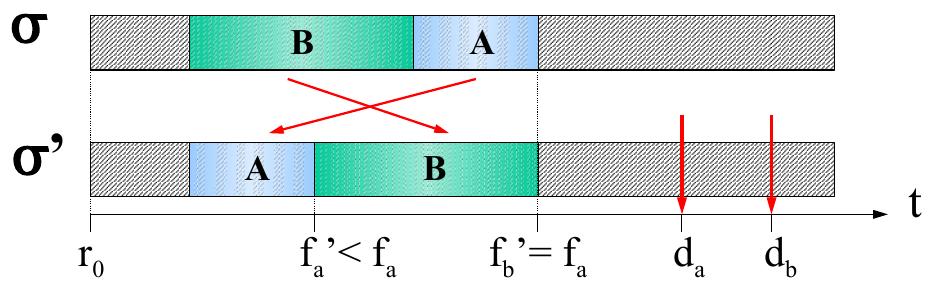
\includegraphics[width=0.4\textwidth]{img/edd_opt}
\end{figure}